\documentclass[aps,prx,twocolumn,superscriptaddress,nofootinbib,longbibliography]{revtex4-2}

\usepackage{amsmath,amssymb,graphicx,bm}
\usepackage[colorlinks=true,linkcolor=blue,citecolor=blue,urlcolor=blue]{hyperref}
\usepackage{booktabs}
\usepackage{amsthm}
\theoremstyle{plain}
\newtheorem{theorem}{Theorem}
\newtheorem{proposition}{Proposition}
\newtheorem{corollary}{Corollary}

\newcommand{\vecop}{\operatorname{vec}}
\newcommand{\Tr}{\operatorname{Tr}}
\newcommand{\ket}[1]{|#1\rangle}
\newcommand{\bra}[1]{\langle#1|}
\newcommand{\adj}{^{\dagger}}
\newcommand{\norm}[1]{\lVert#1\rVert}

\begin{document}

\title{Open-system dynamics on a single continuous quantum circuit\\
       with a classical cost independent of the number of time steps}

\author{Simon Mader}
\affiliation{Preprint draft --- affiliation to be completed}

\date{\today}

\begin{abstract}
Dilation-based quantum simulation of open quantum systems has a structural
weakness that is rarely stated plainly: in essentially every published scheme
the classical computer must first produce a substantial part of the answer ---
a sequence of dynamical maps, a memory kernel, or a window of past states ---
before the quantum circuit can run at all, and the amount of that classical work
grows with the length of the simulation.  We remove this dependence.  For
Markovian evolution a Stinespring dilation turns the channel into one fixed
unitary followed by an environment reset; nothing is measured, nothing is
re-prepared, and the circuit is deterministic.  For non-Markovian evolution we
observe that the hierarchical equations of motion (HEOM) already form a closed
linear system, so that the exact propagator on the auxiliary-density-operator
(ADO) space needs no memory kernel and no memory length $K$.  The single
obstruction is that this propagator has spectral radius exactly one but operator
norm $32.4$ for the four-site FMO model, which destroys any step-wise Sz.-Nagy
dilation because post-selection probabilities multiply.  We show that this is a
property of the inner product rather than of the physics, and remove it in two
independent ways: a Lyapunov metric in which the generator is dissipative, and
the physical rescaling of the ADOs, which alone reduces the operator norm from
$7.7\times10^{5}$ to $1.02$ at strong coupling.  A Krylov compression is then
contractive by construction, and the whole evolution runs as one gate repeated
on eight qubits with post-selection probability one.  Measured against QuTiP's
HEOM solver, the circuit reproduces the four-site FMO dynamics to
$4\times10^{-7}$ over $1$~ps and $4.7\times10^{-6}$ over $10$~ps, with zero
classically propagated time steps.  We also state carefully what the method does
\emph{not} deliver: no quantum advantage, a gate that is far beyond present
hardware, and a read-out whose cost is not accounted for.
\end{abstract}

\maketitle

\section{Introduction}

Simulating an open quantum system on a quantum computer means implementing a
non-unitary map with unitary hardware.  The standard tool is dilation: enlarge
the Hilbert space until the map becomes the restriction of a unitary.  Both
classical constructions are old --- Stinespring's for completely positive maps
\cite{Stinespring1955} and Sz.-Nagy's for contractions \cite{SzNagy1953} --- and
both have been used repeatedly to put open-system dynamics onto circuits.

There is, however, a recurring and under-advertised catch.  A dilation can only
be built from a matrix that is already known.  In practice this means the
classical computer must first generate the object to be dilated, and in the
non-Markovian case that object is usually a \emph{sequence}: the dynamical maps
$\mathcal E_1,\dots,\mathcal E_K$, the transfer tensors derived from them
\cite{Cerrillo2014}, or a window of past reduced states.  The length $K$ of that
sequence controls the accuracy, so improving the result means computing more of
the trajectory classically --- exactly the work the quantum computer was
supposed to do.  For the four-site Fenna--Matthews--Olson (FMO) model studied
below, reaching an accuracy of $9\times10^{-4}$ over $100$ steps by the
transfer-tensor route requires $40$ of those $100$ steps to be produced
classically first.

This paper removes that dependence.  The central claim is narrow and we state it
precisely, because a looser version of it would be wrong:

\begin{quote}
\emph{The classical work is $O(1)$ in the number of time steps $n$ and in the
total simulated time $T$.  A fixed, $n$-independent set-up produces one unitary,
and the circuit then runs for arbitrarily many steps by repeating it.}
\end{quote}

We emphasise what this does not say.  It does not say the classical work is
small --- it is $O(\mathcal D^3)$ in the dimension $\mathcal D$ of the extended
space, and for the model treated here it is in fact slower than solving the
equations of motion outright.  It does not claim a quantum advantage.  What it
does say is that the classical and quantum parts have been cleanly separated:
the classical side pays once, and the number of time steps is thereafter carried
entirely by the circuit.

Section~\ref{sec:markov} treats the Markovian case, where the construction is
deterministic and the post-selection problem does not arise at all.
Section~\ref{sec:nonmarkov} treats the non-Markovian case, where it does, and
constitutes the main body of the paper.  Section~\ref{sec:results} reports
measurements against QuTiP's HEOM solver \cite{Lambert2023,Johansson2013}, and
Section~\ref{sec:limits} states the limitations.

\section{Markovian evolution: one gate and a reset}
\label{sec:markov}

Let $\Phi$ be a completely positive trace-preserving (CPTP) map on a
$d$-dimensional system with Kraus operators $\{M_k\}_{k=1}^{K}$, so that
$\sum_k M_k\adj M_k = \mathbb 1$.  Introduce an environment
$\mathcal H_E\cong\mathbb C^{K}$ with orthonormal basis $\{\ket{k}\}$ and define
\begin{equation}
V:\mathcal H\to\mathcal H_E\otimes\mathcal H,\qquad
V\ket{\psi}=\sum_{k=1}^{K}\ket{k}_E\otimes M_k\ket{\psi}.
\label{eq:V}
\end{equation}

\begin{proposition}
$V$ is an isometry, and $\Tr_E[V\rho V\adj]=\Phi(\rho)$ for every state $\rho$.
\end{proposition}

\begin{proof}
For the first claim,
$\bra{\varphi}V\adj V\ket{\psi}
 =\sum_{k,k'}\langle k|k'\rangle\,\bra{\varphi}M_k\adj M_{k'}\ket{\psi}
 =\bra{\varphi}\big(\sum_k M_k\adj M_k\big)\ket{\psi}
 =\langle\varphi|\psi\rangle$,
using trace preservation in the last step.  For the second, expanding
$V\rho V\adj=\sum_{k,k'}\ket{k}_E\bra{k'}_E\otimes M_k\rho M_{k'}\adj$ and
tracing over $E$ gives
$\sum_j\sum_{k,k'}\langle j|k\rangle\langle k'|j\rangle\,M_k\rho M_{k'}\adj
 =\sum_k M_k\rho M_k\adj=\Phi(\rho)$.
\end{proof}

Because the columns of $V\in\mathbb C^{N\times d}$ ($N=Kd$) are orthonormal, they
can be completed by $N-d$ further orthonormal columns to a unitary
$U\in\mathrm U(N)$ whose first $d$ columns are those of $V$.  Since
$\ket{0}_E\otimes\ket{\psi}$ is supported only on those first $d$ coordinates,
$U(\ket{0}_E\otimes\ket{\psi})=V\ket{\psi}$, and therefore
\begin{equation}
\rho_n=\Phi(\rho_{n-1})
      =\Tr_E\!\Big[U\big(\ket{0}\bra{0}_E\otimes\rho_{n-1}\big)U\adj\Big].
\label{eq:stinespring-step}
\end{equation}

Equation~\eqref{eq:stinespring-step} is the entire Markovian algorithm.  One
fixed gate $U$ acts on environment plus system; the partial trace is realised on
hardware by resetting the environment register.  Nothing is measured, nothing is
post-selected, nothing is re-prepared between steps, and iterating $n$ times
gives $\Phi^n(\rho_0)$ exactly.  The success probability is $1$ by construction.

For the four-site FMO model with a Lindblad generator this yields $2$ system
qubits, $4$ environment qubits and $16$ Kraus operators; the circuit is $100$
applications of one gate interleaved with resets.  The single classical input is
the Kraus set of the \emph{one-step} channel $\Phi(\Delta t)$, computed once.

The reason this is so easy is precisely the reason it does not generalise: a
fixed CPTP map iterated on the system alone is a semigroup, hence Markovian.
Non-Markovian evolution therefore requires either a coherent memory register or
non-trace-preserving operations, i.e.\ post-selection.  We now take the first
route, and the post-selection appears as the price of the dilation rather than
of the physics.

\section{Non-Markovian evolution}
\label{sec:nonmarkov}

\subsection{HEOM is already a closed linear system}

In the hierarchical equations of motion \cite{Tanimura1989,Tanimura2020} the
reduced density matrix is propagated together with a set of auxiliary density
operators (ADOs) that carry the bath correlations.  Stacking them into one
vector
\begin{equation}
\vec\Sigma(\tau)=\big(\vecop\rho_S,\;\vecop\rho_{\mathbf n_1},\;\dots\big)
\in\mathbb C^{\mathcal D},\quad \mathcal D=N_{\rm ADO}\,d^2,
\end{equation}
the evolution is local in time,
$\partial_\tau\vec\Sigma=\mathcal L\,\vec\Sigma$, with a time-independent
$\mathcal L$.  With $P=e^{\mathcal L\Delta\tau}$ and the projector
$\Pi=[\mathbb 1_{d^2}\;0\;\cdots\;0]$ onto the zeroth ADO,
\begin{equation}
\boxed{\;\vecop\rho_S(k\Delta\tau)=\Pi\,P^{\,k}\,\vec\Sigma(0)
\quad\text{exactly, for every }k.\;}
\label{eq:exact}
\end{equation}

\begin{proposition}
On the extended space the evolution is a semigroup; all non-Markovianity of
$\rho_S$ arises from $\Pi$ not being invertible.  In particular no memory length
$K$ appears.
\end{proposition}

\begin{proof}
$\mathcal L$ is time-independent, so
$e^{\mathcal L(\tau+\sigma)}=e^{\mathcal L\tau}e^{\mathcal L\sigma}$ and
$\vec\Sigma_k=P\vec\Sigma_{k-1}$ depends on its immediate predecessor only.  The
reduced maps $\mathcal E_k=\Pi P^k\Pi^{\mathsf T}$ fail to compose because
$\Pi^{\mathsf T}\Pi=\mathrm{diag}(\mathbb 1_{d^2},0,\dots,0)\neq\mathbb 1$ ---
projecting onto the system block \emph{deletes} the bath memory that the ADOs
were carrying.
\end{proof}

This is the point at which the transfer-tensor construction gives away more than
it needs to.  It starts one level below Eq.~\eqref{eq:exact}, from the reduced
maps $\mathcal E_k$, inverts the convolution to obtain transfer tensors $T_m$,
and truncates the resulting sum at $K$ terms.  Both of its costs --- the
discarded correlations beyond $K\Delta t$ and the $K$ classically propagated
states needed to fill the history window --- are consequences of having
projected in the first place.  Keeping the ADOs costs a larger vector and
removes $K$ entirely.

\subsection{The obstruction: a bounded trajectory with a large operator norm}

Dilating $P$ directly fails, and it is worth being precise about why.  For a
matrix $M$ with $\norm{M}_2\le s$, the Sz.-Nagy dilation
\begin{equation}
U=\begin{pmatrix}
M/s & \sqrt{\mathbb 1-MM\adj/s^2}\\
\sqrt{\mathbb 1-M\adj M/s^2} & -(M/s)\adj
\end{pmatrix}
\label{eq:sznagy}
\end{equation}
is unitary, and projecting one ancilla onto $\ket{0}$ after each of $n$
applications succeeds with probability
\begin{equation}
p_n=\frac{\norm{M^{\,n}x}^2}{s^{2n}\norm{x}^2}.
\label{eq:psucc}
\end{equation}
The denominator is a worst case over the whole space applied $n$ times, while
the numerator follows the one trajectory that is actually taken.  For the
four-site FMO HEOM generator at $\Delta t=10$~fs we measure
$\rho(P)=1.000000$ but $\norm{P}_2=32.39$, so $s^{2n}=32.39^{200}\approx10^{301}$.

Refining the time step does not help.

\begin{proposition}
Let $T=n\Delta\tau$ be fixed and $s(\Delta\tau)=\norm{e^{\mathcal L\Delta\tau}}_2$.
Then $n\ln s(\Delta\tau)\to T\,\omega(\mathcal L)$ as $\Delta\tau\to0$, where
$\omega(\mathcal L)=\lambda_{\max}\big(\tfrac12(\mathcal L+\mathcal L\adj)\big)$
is the numerical abscissa.
\end{proposition}

\begin{proof}
With $x(\tau)=e^{\mathcal L\tau}x_0$,
$\tfrac{d}{d\tau}\norm{x}^2=2\,x\adj\tfrac12(\mathcal L+\mathcal L\adj)x
\le2\omega\norm{x}^2$, with equality for the top eigenvector of the Hermitian
part.  Hence $s(\Delta\tau)=1+\omega\Delta\tau+O(\Delta\tau^2)$ and
$n\ln s=\tfrac{T}{\Delta\tau}(\omega\Delta\tau+O(\Delta\tau^2))\to T\omega$.
\end{proof}

We measure $\omega(\mathcal L)=+2.61\times10^{3}\,\mathrm{cm}^{-1}$ and
$T=0.1884\,\mathrm{cm}$, giving $T\omega\approx4.9\times10^{2}$ and
$p\approx e^{-984}$ irrespective of the discretisation.  The gap between
$\rho(P)=1$ and $\norm{P}_2=32$ is the familiar signature of a strongly
non-normal operator \cite{Trefethen2005}.

It is instructive that the trajectory itself is not bounded either, but in the
opposite direction: along the physical path
$\norm{P^n\vec\Sigma_0}/\norm{\vec\Sigma_0}$ rises to a maximum of $3165$ and
sits at $1101$ after $100$ steps.  Both factors in Eq.~\eqref{eq:psucc} are
therefore absurd --- $8.2\times10^{-303}$ and $1.2\times10^{6}$ --- and they very
nearly, but not nearly enough, cancel.  The reason is that only
$5.2\times10^{-4}$ of $\norm{\vec\Sigma_{100}}$ belongs to the system block; the
rest lives in the ADOs, which are bookkeeping objects rather than density
matrices and are under no obligation to stay bounded.  The Euclidean norm is
simply the wrong yardstick on this space.

\subsection{A metric in which the generator is dissipative}

\begin{theorem}[Lyapunov gauge]
Let $\delta>0$ be such that $\mathcal L-\delta\mathbb 1$ is Hurwitz.  Then
\begin{equation}
(\mathcal L-\delta\mathbb 1)\adj W+W(\mathcal L-\delta\mathbb 1)=-\mathbb 1
\label{eq:lyap}
\end{equation}
has a unique solution, it is Hermitian positive definite, and
$\norm{e^{\mathcal L\tau}}_W\le e^{\delta\tau}$ for all $\tau\ge0$, where
$\norm{x}_W=\norm{W^{1/2}x}_2$.
\end{theorem}

\begin{proof}
Set $W=\int_0^\infty\big(e^{(\mathcal L-\delta)\tau}\big)\adj
e^{(\mathcal L-\delta)\tau}\,d\tau$.  The integral converges because
$\mathcal L-\delta$ is Hurwitz, and $x\adj Wx=\int_0^\infty
\norm{e^{(\mathcal L-\delta)\tau}x}^2d\tau>0$ gives positive definiteness.
Differentiating the integrand and integrating from $0$ to $\infty$ yields
Eq.~\eqref{eq:lyap}, the boundary term at infinity vanishing and the one at zero
giving $-\mathbb 1$.  Uniqueness holds because the Sylvester operator
$X\mapsto(\mathcal L-\delta)\adj X+X(\mathcal L-\delta)$ has eigenvalues
$\bar\lambda_i+\lambda_j$ with strictly negative real part.  Finally, with
$V(\tau)=x(\tau)\adj Wx(\tau)$ and $\dot x=\mathcal Lx$,
\begin{equation*}
V'=x\adj(\mathcal L\adj W+W\mathcal L)x
  =x\adj(-\mathbb 1+2\delta W)x\le2\delta V,
\end{equation*}
and Gr\"onwall gives $V(\tau)\le e^{2\delta\tau}V(0)$.
\end{proof}

The shift is needed only because $\mathcal L$ has the stationary state as an
exact zero eigenvalue, which would make the integral diverge along that one
direction.

\begin{corollary}
$\tilde P=W^{1/2}PW^{-1/2}$ satisfies $\norm{\tilde P}_2\le e^{\delta\Delta\tau}$
and is similar to $P$.  The gauge therefore introduces no approximation
whatsoever: $\tilde P^{\,k}=W^{1/2}P^kW^{-1/2}$ and
$\vecop\rho_S(k\Delta\tau)=\Pi W^{-1/2}\tilde P^{\,k}\tilde{\vec\Sigma}_0$.
\end{corollary}

Read with $s=e^{\delta\Delta\tau}$, Eq.~\eqref{eq:psucc} becomes
$p_n=e^{-2\delta T}\norm{\tilde P^n\tilde{\vec\Sigma}_0}^2/\norm{\tilde{\vec\Sigma}_0}^2$,
which is $O(1)$.  Measured: $\norm{P}_2=32.39\to\norm{\tilde P}_2=1.000038$ and
$p_{100}$ from $9.9\times10^{-297}$ to $0.365$, a ratio of $3.7\times10^{295}$
(Fig.~\ref{fig:gauge}).

\begin{figure}[t]
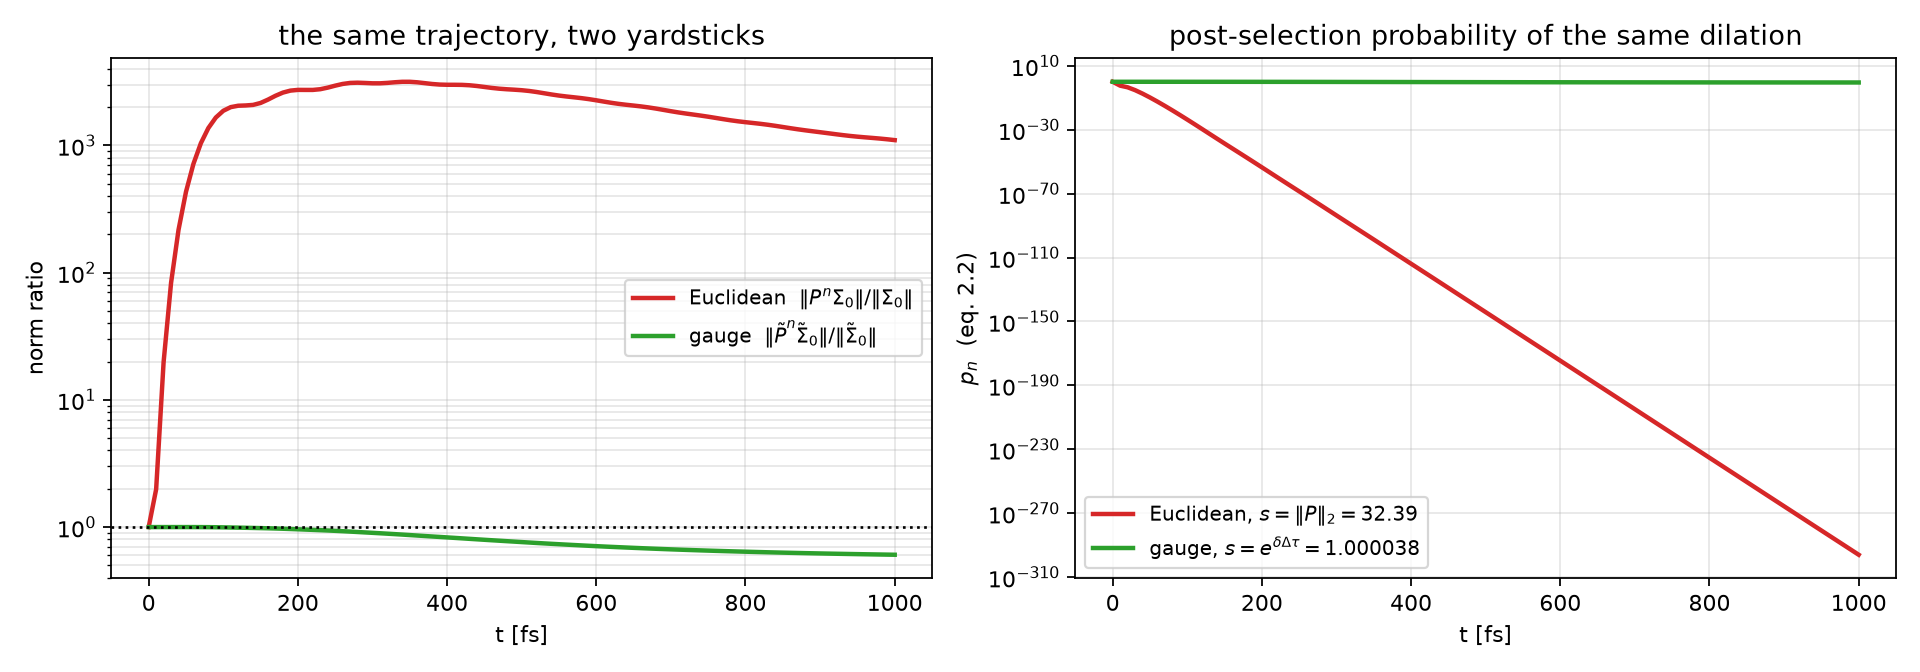
\includegraphics[width=\columnwidth]{figures/gauge_postselection_N4.png}
\caption{The same physical trajectory measured with two yardsticks.  Left: the
Euclidean norm of the ADO vector grows by three orders of magnitude, because
almost all of it belongs to the auxiliary operators rather than to $\rho_S$; in
the gauge it is a contraction.  Right: the post-selection probability of the
identical Sz.-Nagy dilation, $10^{-297}$ against $0.365$.}
\label{fig:gauge}
\end{figure}

\subsection{Attacking the cause: rescaling the ADOs}

The gauge treats the symptom.  The cause is that the ADOs, in the conventional
HEOM normalisation, differ enormously in magnitude: the operator with
multi-index $\mathbf n$ carries a prefactor $\prod_k c_k^{n_k}$, and the bath
coefficients $c_k$ span orders of magnitude.  A unit step in a deep ADO means
something numerically very different from a unit step in $\rho_S$, and the
transient growth of $\norm{P}_2$ is precisely the propagator moving weight from
small-scale to large-scale coordinates.

The standard remedy \cite{Shi2009} is the diagonal rescaling
\begin{equation}
\tilde\rho_{\mathbf n}
 =\frac{\rho_{\mathbf n}}{\sqrt{\prod_k n_k!\,|c_k|^{n_k}}}
\;\Longleftrightarrow\;
\tilde{\mathcal L}=D^{-1}\mathcal L D,
\label{eq:adoscale}
\end{equation}
a similarity transformation and hence exact.  The zeroth ADO carries the factor
$1$, so neither the initial state nor the read-out is affected.  Its effect is
striking (Table~\ref{tab:scaling}): the operator norm falls from
$7.7\times10^{5}$ to $1.023$ at $\lambda=100\,\mathrm{cm}^{-1}$.  The
``norm catastrophe'' is thus largely an artefact of the coordinate convention.
We note that QuTiP~5 does not apply this rescaling.

\begin{table}[t]
\caption{Effect of the ADO rescaling~\eqref{eq:adoscale} on the operator norm of
the one-step propagator, four-site FMO, $\Delta t=10$~fs, hierarchy depth $3$.}
\label{tab:scaling}
\begin{ruledtabular}
\begin{tabular}{cccc}
$\lambda$ (cm$^{-1}$) & $\norm{P}_2$ raw & $\norm{P}_2$ rescaled & spread $s_{\max}/s_{\min}$\\
\colrule
$3$   & $32.39$              & $1.001$ & $1.08\times10^{5}$\\
$35$  & $3.12\times10^{4}$   & $1.017$ & $4.18\times10^{6}$\\
$100$ & $7.71\times10^{5}$   & $1.023$ & $2.07\times10^{7}$\\
\end{tabular}
\end{ruledtabular}
\end{table}

Rescaling alone is not sufficient --- $1.023^{200}\approx10^{2}$ would still be
fatal, and $\rho(P)=1$ still forces $\delta>0$ --- but it leaves the gauge only a
residual correction to make, with a condition number many orders of magnitude
smaller.  A blind numerical alternative is not a substitute: balancing the
generator with \texttt{scipy.linalg.matrix\_balance} reaches only
$\norm{P}_2=2.54$ at $\lambda=3$ and achieves nothing at all at $\lambda=100$.

\subsection{Krylov compression becomes free}

The gauged propagator still acts on $\mathbb C^{2640}$.  Compress it onto the
Krylov space $\mathcal K_m(\tilde P,\tilde{\vec\Sigma}_0)$ with an orthonormal
Arnoldi basis $Q_m$ \cite{Saad1992},
$\tilde P Q_m=Q_mH_m+h_{m+1,m}q_{m+1}e_m^{\mathsf T}$,
$H_m=Q_m\adj\tilde PQ_m$.

\begin{proposition}
$\norm{H_m}_2\le\norm{\tilde P}_2$ for every $m$.
\end{proposition}

\begin{proof}
$Q_m$ is an isometry, so
$\norm{H_my}=\norm{Q_m\adj\tilde PQ_my}\le\norm{\tilde PQ_my}
\le\norm{\tilde P}\norm{y}$.
\end{proof}

This is why the gauge must come first.  Compressing the raw $P$ gives
$\norm{H_m}\approx32$ and a trajectory that diverges to $10^{65}$; compressing
$\tilde P$ gives a contraction for \emph{every} $m$, so $m$ ceases to be a
trade-off and becomes a pure convergence parameter, costing
$\lceil\log_2m\rceil$ qubits and nothing else.  Moreover $H_m^{\,k}Q_m\adj
\tilde{\vec\Sigma}_0=Q_m\adj\tilde P^{\,k}\tilde{\vec\Sigma}_0$ for $k\le m-1$,
so the first $m$ steps are exact.

\subsection{The circuit}

$H_m$ is padded to $m_p=2^{\lceil\log_2m\rceil}$ and dilated once by
Eq.~\eqref{eq:sznagy} into a single unitary on $\lceil\log_2m\rceil+1$ qubits.
No state preparation is required: by construction of the Arnoldi basis the
initial vector is $\norm{\tilde{\vec\Sigma}_0}e_1$, so the register starts in
$\ket{0\cdots0}$.  Each step applies $U$, measures the ancilla into its own
classical bit and resets it; the run is accepted if the record is all zeros.

\begin{proposition}
Conditioned on the record $0\cdots0$, the register state after $t$ steps is
$H_m^{\,t}y_0/\norm{H_m^{\,t}y_0}$, independent of any randomness in the
measurements.
\end{proposition}

\begin{proof}
By induction.  If the register is in the pure state $\ket{y_{t-1}}\ket{0}_E$,
Eq.~\eqref{eq:sznagy} gives
$U\ket{y_{t-1}}\ket{0}=(M_s\ket{y_{t-1}})\ket{0}+(D\ket{y_{t-1}})\ket{1}$ with
$M_s=H_m/s$.  Obtaining $0$ projects onto the first summand, and renormalisation
cancels $1/s$, leaving $H_m\ket{y_{t-1}}/\norm{H_m y_{t-1}}$, a function of
$y_{t-1}$ alone.  The reset restores the hypothesis.
\end{proof}

The outcome record is random; the state conditioned on it is not.  One accepted
shot therefore already carries the exact state, and statistics are needed only
for the scalar $p_t$, which supplies the norm through
$\norm{y_t}=s^t\sqrt{p_t}\norm{y_0}$.  Alternatively, trace preservation
$\Tr\rho_S(t)=1$ fixes the same scalar without any statistics.  This also
dictates how the circuit must be simulated: Qiskit Aer samples mid-circuit
measurements in the density-matrix method exactly as in the statevector method,
so reading the post-selected branch out of a saved density matrix is
Monte-Carlo, whereas \texttt{save\_statevector(conditional=True)} returns the
accepted branch itself.

\section{Results}
\label{sec:results}

All numbers are for the four-site FMO Hamiltonian with one Drude--Lorentz Pad\'e
bath per site, $\gamma=50\,\mathrm{cm}^{-1}$, $T=300$~K, $\Delta t=10$~fs,
hierarchy depth $3$ ($165$ ADOs, $\mathcal D=2640$), and are measured against
QuTiP's \texttt{HEOMSolver} \cite{Lambert2023} and nothing else.

\begin{figure}[t]
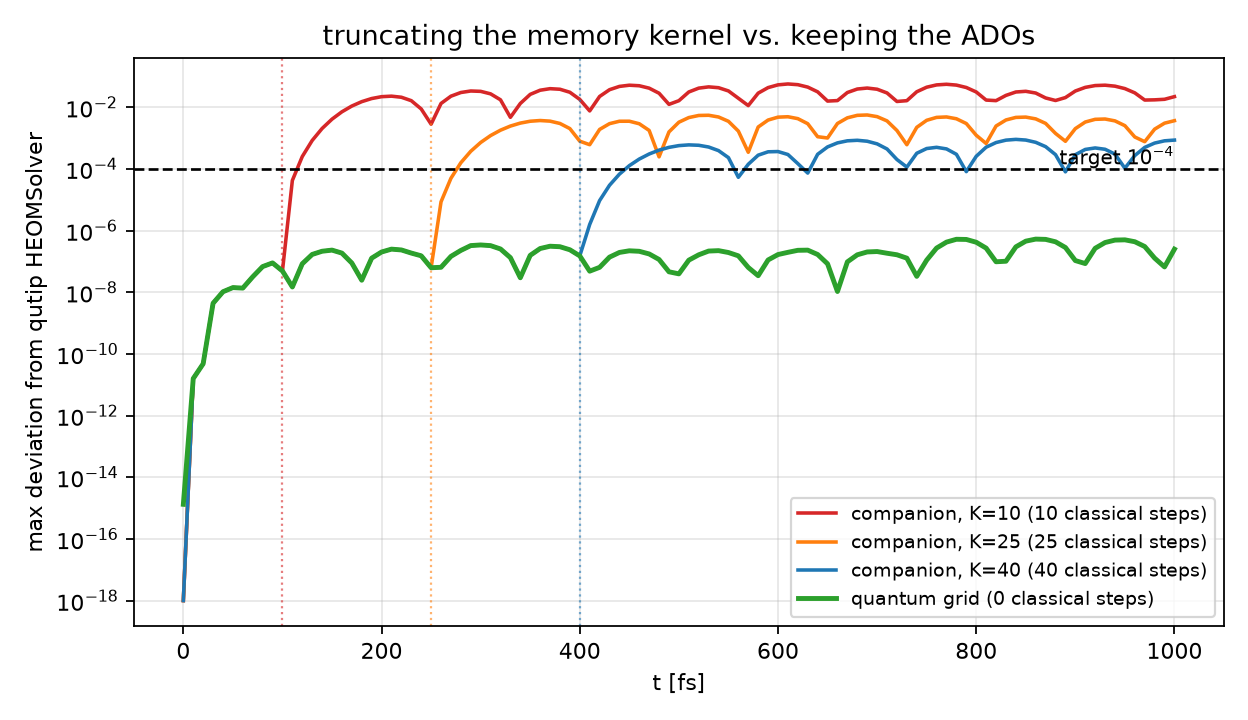
\includegraphics[width=\columnwidth]{figures/vs_companion_N4.png}
\caption{Deviation from the exact solver over $100$ steps.  The transfer-tensor
route (coloured) improves only by moving more of the trajectory onto the
classical computer; the vertical dotted lines mark where each history window
ends.  The present method (green) uses none.}
\label{fig:companion}
\end{figure}

\paragraph{Against the transfer-tensor route.}
At $\lambda=3\,\mathrm{cm}^{-1}$ over $100$ steps, the companion operator gives
$5.66\times10^{-2}$, $5.58\times10^{-3}$ and $9.03\times10^{-4}$ for $K=10$, $25$
and $40$, requiring $10$, $25$ and $40$ classically propagated steps
respectively.  Iterating the ADO propagator gives $5.27\times10^{-7}$ with none
(Fig.~\ref{fig:companion}).  That floor is the reference solver's own
integration tolerance: propagating the full $2640\times2640$ matrix with neither
gauge nor compression reproduces the identical figure.

\paragraph{Convergence in $m$.}
With $\delta=0.02$: $m=16$ gives $1.93\times10^{-1}$ ($5$ qubits), $m=32$ gives
$6.22\times10^{-2}$ ($6$), and $m\ge64$ gives $5.27\times10^{-7}$ ($7$ qubits),
with $\norm{H_m}_2=1.000038$ independent of $m$ as required.  Against the exact
gauged trajectory the compression error at $m=128$ is $1.9\times10^{-14}$ over
$100$ steps and $1.65\times10^{-8}$ over $500$.

\paragraph{Long runs.}
Since $\norm{H_m}_2\le e^{\delta\Delta\tau}$, the iteration cannot blow up.  Over
$100$, $500$ and $1000$ steps the circuit reproduces the solver to
$4.99\times10^{-7}$, $1.85\times10^{-6}$ and $4.65\times10^{-6}$, with the
post-selection probability settling into a plateau rather than decaying
(Fig.~\ref{fig:long}).  The error grows sub-linearly and saturates; the density
matrix stays trace-preserving to $2.4\times10^{-9}$ and positive semidefinite to
$-2\times10^{-15}$ over $5$~ps.  The circuit itself adds nothing: it reproduces
the classical iteration of $H_m$ to $7.7\times10^{-10}$.

\begin{figure}[t]

\includegraphics[width=\columnwidth]{figures/long_run_N4.png}
\caption{Populations from the circuit over $500$ applications of the same gate
(left) and the deviation from the exact solver together with the post-selection
probability (right).}
\label{fig:long}
\end{figure}

\paragraph{The shift $\delta$.}
The naive expectation is that $\delta$ costs only $e^{-2\delta T}$ and is
otherwise irrelevant.  That is incomplete, because $W$ itself depends on
$\delta$: the smaller $\delta$, the more weight the metric places on the
stationary state, towards which the trajectory relaxes, so the state loses
almost no length in that metric.  Measured $p_{100}$: $0.1995$ at $\delta=10^{-1}$,
$0.8896$ at $10^{-3}$, and $1.0000$ at $10^{-7}$, while $e^{-2\delta T}$ moves
only from $0.963$ to $1.000$.  Below that, $\mathrm{cond}(W)$ grows as
$1/\delta$; at $\delta=10^{-11}$ it reaches $2.1\times10^{19}$, the guarantee
$\norm{\tilde P}_2\le e^{\delta\Delta\tau}$ is violated ($3.56$ measured), and
$p$ collapses to zero.  The practical rule is to reduce $\delta$ until $p\approx1$
and no further; comparing the measured norm against the guaranteed bound is a
free validity check.

\paragraph{Coupling strength.}
Table~\ref{tab:sweep} shows the range.  Without rescaling the method fails
between $\lambda=3$ and $\lambda=100$.  With it, everything up to
$\lambda=300\,\mathrm{cm}^{-1}$ runs with $\norm{\tilde P}_2=1.000000$ and
$p=1.0000$, and $\mathrm{cond}(W)$ grows only linearly in $\lambda$ rather than
quadratically.  At $\lambda=1000$ the calculation fails even with rescaling ---
but for a structural reason: the spectral abscissa of the depth-$3$ generator is
$+3.70\,\mathrm{cm}^{-1}$, so the truncated hierarchy is genuinely unstable, no
positive definite $W$ exists, and the reference solver is equally meaningless
there.  The cure is a deeper hierarchy, not better linear algebra.  For
comparison, the physically relevant FMO value is $\lambda\approx35$.

\begin{table}[t]
\caption{Coupling sweep, $100$ steps, $\delta=10^{-5}$, $m=128$.  ``Guarantee''
is the check $\norm{\tilde P}_2\le e^{\delta\Delta\tau}$.  At $\lambda=1000$ the
generator itself is unstable (spectral abscissa $+3.70$).}
\label{tab:sweep}

\begin{ruledtabular}
\begin{tabular}{ccccc}
$\lambda$ & resc. & $\mathrm{cond}(W)$ & vs.\ solver & $p_{100}$\\
\colrule
$3$    & no  & $2.87\times10^{13}$ & $5.27\times10^{-7}$ & $0.9987$\\
$3$    & yes & $6.78\times10^{8}$  & $5.27\times10^{-7}$ & $1.0000$\\
$100$  & no  & $4.09\times10^{22}$ & $5.80\times10^{-8}$ & $0$\\
$100$  & yes & $1.60\times10^{9}$  & $5.79\times10^{-8}$ & $1.0000$\\
$300$  & no  & \multicolumn{3}{c}{$W$ not pos. def.}\\
$300$  & yes & $6.79\times10^{9}$  & $2.00\times10^{-8}$ & $1.0000$\\
$1000$ & yes & \multicolumn{3}{c}{gen. unstable}\\
\end{tabular}
\end{ruledtabular}
\end{table}

\section{Where the work happens}
\label{sec:cost}

Table~\ref{tab:cost} is the point of the paper.  Every classical step is
performed once and none of them scales with $n$ or $T$.

\begin{table}[t]
\caption{Cost of the non-Markovian construction.  $\mathcal D=N_{\rm ADO}d^2$ is
the ADO-space dimension, $m$ the Krylov dimension, $n$ the number of steps.}
\label{tab:cost}
\begin{ruledtabular}
\begin{tabular}{lcc}
step & cost & grows with $n$?\\
\colrule
assemble $\mathcal L$ & sparse & no\\
Lyapunov solve~\eqref{eq:lyap} & $O(\mathcal D^3)$ & no\\
$P=e^{\mathcal L\Delta\tau}$ & $O(\mathcal D^3)$ & no\\
Arnoldi & $m$ matvecs & no\\
dilation~\eqref{eq:sznagy} & $O(m^3)$ & no\\
\textbf{propagation} & $n\times$ one gate & \textbf{on the circuit}\\
\end{tabular}
\end{ruledtabular}
\end{table}

The comparison that matters is with the alternatives.  The transfer-tensor route
pays $K$ propagation steps before the circuit starts, and $K$ must grow with $n$
to hold the accuracy; a direct classical solve pays all $n$.  Here the classical
side pays a fixed $O(\mathcal D^3)$ and the same $m=128$ carries $100$, $500$ and
$1000$ steps without modification.

One qualification is required, and it is the one a careful reader will raise
first.  The Krylov space
$\mathcal K_m=\mathrm{span}\{\tilde{\vec\Sigma}_0,\tilde P\tilde{\vec\Sigma}_0,
\dots,\tilde P^{m-1}\tilde{\vec\Sigma}_0\}$ \emph{contains} the first $m$ time
steps, and building it costs $m$ matrix--vector products.  For $n\lesssim m$ the
method therefore saves nothing at all.  The claim that survives is the scaling
one: $m$ does not depend on $n$, whereas $K$ does.

\section{What this does not do}
\label{sec:limits}

We list the limitations plainly, because several of them are severe.

\emph{No quantum advantage.}  The set-up takes $122$~s against the reference
solver's $0.27$~s for the same answer.  The circuit performs the cheapest part of
the problem --- repeatedly applying a small, already-known matrix.  The result
demonstrates that exact non-Markovian dynamics \emph{fits} on a continuous
circuit, not that doing so is currently worthwhile.

\emph{The gate is not hardware-executable.}  $U$ is a dense $256\times256$
matrix without structure; a Quantum Shannon decomposition \cite{Shende2006}
needs $\sim\!3\times10^{4}$ CNOTs per application and $\sim\!3\times10^{6}$ for
$100$ steps, far beyond present coherence times.  We measured $94$, $423$ and
$1783$ CNOTs at $4$, $5$ and $6$ qubits, consistent with the $\tfrac{23}{48}4^{n}$
scaling.

\emph{The read-out is not priced in.}  $\vecop\rho_S=Ry_t$ is a linear functional
of the register state, not an observable, and on hardware would require
tomography of the Krylov register or a Hadamard test per component.  This gap is
shared with the transfer-tensor route.

\emph{Accuracy is measured against the same truncation.}  Our $5\times10^{-7}$ is
the distance to QuTiP at depth $3$ and $N_k=1$, not to the physics.  Depth $4$
against depth $3$ differs by $2.3\times10^{-3}$ (whereas $N_k=2$ against $N_k=1$
differs by only $1.2\times10^{-5}$), so the hierarchy truncation --- shared with
the reference --- dominates the real error budget by four orders of magnitude.

\emph{Memory.}  The Lyapunov solve needs several dense
$\mathcal D\times\mathcal D$ matrices.  Seven sites at depth $2$ ($\mathcal D=5880$)
is feasible; at depth $3$ ($\mathcal D=33\,320$, $\sim\!18$~GB per matrix) it is
not.  Replacing the dense solve by a low-rank method is the obvious next step,
with the caveat that low-rank solvers return a singular $W$, which is not
directly usable as a metric.

\emph{State dependence.}  The gauge $W$ is universal and is reused, but the
Krylov basis is not: a different initial state requires a fresh Arnoldi run
(no new Lyapunov solve and no new exponential).  The grid is therefore not a
universal propagator in the sense of a dynamical map.

\section{Conclusion}

For Markovian evolution, a Stinespring dilation gives a deterministic circuit:
one fixed gate, an environment reset, no measurement and unit success
probability.  For non-Markovian evolution, the auxiliary density operators
already carry the full memory, so the exact propagator requires no memory kernel
and no memory length; the only obstruction is that this propagator has operator
norm $32$ while its spectral radius is $1$, and that obstruction lives in the
inner product rather than in the physics.  A Lyapunov metric removes it exactly,
the physical ADO rescaling removes most of it at its source, and a Krylov
compression is then contractive by construction.  What remains is one gate on
eight qubits, repeated, with post-selection probability one and agreement with
the exact solver at the level of that solver's own tolerance.

The classical cost of the construction is independent of the number of time
steps.  That is a structural statement about where the work sits, not a
performance claim: the constant is large, and the resulting gate is far beyond
current hardware.  The natural continuations are a sparse or low-rank Lyapunov
solver, which would lift the memory ceiling, and a block-encoding of
$\mathcal L$ that never forms $P$ or $W$ densely --- in which case the
contraction gauge would remain necessary, since the norm problem it solves does
not depend on how the gate is built.

\begin{acknowledgments}
This work builds on the Kraus-operator route to non-Markovian dynamics of
Ref.~\onlinecite{Seneviratne2024}.  Numerical reference dynamics were computed
with QuTiP \cite{Johansson2013,Lambert2023}; circuits were built and simulated
with Qiskit \cite{Qiskit}.
\end{acknowledgments}

\bibliographystyle{apsrev4-2}
\bibliography{refs}

\end{document}
